
%(BEGIN_QUESTION)
% Copyright 2011, Tony R. Kuphaldt, released under the Creative Commons Attribution License (v 1.0)
% This means you may do almost anything with this work of mine, so long as you give me proper credit

Anta at den elektriske motoren nekter å gå når ``Run''-trykknappen trykkes, enten hastighetsbryteren står i ``Fast'' eller ``Slow.''  En tekniker starter feilsøking av kretsen, i rekkefølgen vist under:

$$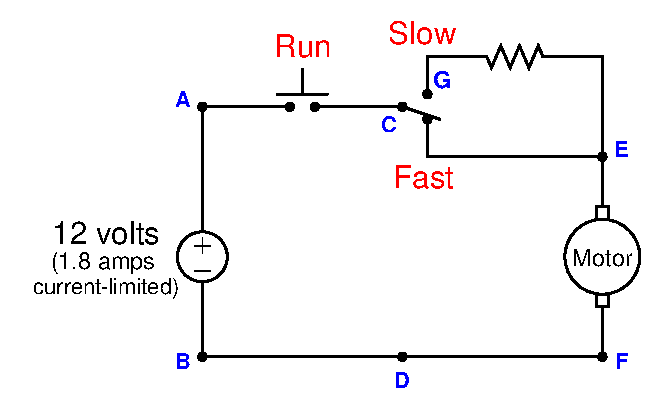
\includegraphics[width=15.5cm]{i00193x01.eps}$$

\begin{itemize}
\item{} {\bf Test 1:} Målt 12 volt DC mellom punkt {\bf A} og {\bf B}, med ``Run''-bryter trykket inn og hastighetsbryter i ``Fast''.
\vskip 25pt
\item{} {\bf Test 2:} Målt 0 volt DC mellom punkt {\bf A} og {\bf C}, med ``Run''-bryter ikke trykket inn og hastighetsbryter i ``Fast''.
\vskip 25pt
\item{} {\bf Test 3:} Målt 12 volt DC mellom punkt {\bf G} og {\bf D}, med ``Run''-bryter trykket inn og hastighetsbryter i ``Fast''.
\vskip 25pt
\item{} {\bf Test 4:} Målt 25 ohm mellom punkt {\bf G} og {\bf E}, med ``Run''-bryter ikke trykket inn og hastighetsbryter i ``Fast''. 
\vskip 25pt
\item{} {\bf Test 5:} Målt 12 volt DC mellom punkt {\bf A} og {\bf F}, med ``Run''-bryter trykket inn og hastighetsbryter i ``Fast''.
\vskip 25pt
\end{itemize}

Identifiser nyttig informasjon om type eller plassering av feilen ut fra resultatene av hver test, i samme rekkefølge som testene ble utført.  Hvis testen ikke er nyttig (dvs. ikke gir ny informasjon), marker den som det.  Anta at det bare er én feil i kretsen, og identifiser plassering og type feil så presist du kan fra testresultatene over.

\vfil 

\underbar{file i00193}
\eject
%(END_QUESTION)





%(BEGIN_ANSWER)

\begin{itemize}
\item{} {\bf Test 1:} Målt 12 volt DC mellom punkt {\bf A} og {\bf B}, med ``Run''-bryter trykket inn og hastighetsbryter i ``Fast''.  {\it Beviser at kilden ikke er død.}
\vskip 5pt
\item{} {\bf Test 2:} Målt 0 volt DC mellom punkt {\bf A} og {\bf C}, med ``Run''-bryter ikke trykket inn og hastighetsbryter i ``Fast''.  {\it Beviser at ``Run''-bryteren ikke har brudd (forutsatt én feil).}
\vskip 5pt
\item{} {\bf Test 3:} Målt 12 volt DC mellom punkt {\bf G} og {\bf D}, med ``Run''-bryter trykket inn og hastighetsbryter i ``Fast''.  {\it Eliminerer alle bruddfeil bortsett fra motoren og ledningen mellom D og F -- feilen må ligge ett av disse to stedene.}
\vskip 5pt
\item{} {\bf Test 4:} Målt 25 ohm mellom punkt {\bf G} og {\bf E}, med ``Run''-bryter ikke trykket inn og hastighetsbryter i ``Fast''.  {\it Unødvendig test, siden vi allerede visste at motstanden ikke hadde brudd fra test 3, og siden feilen må være felles for begge hastighetsposisjoner (motoren går ikke verken i ``Fast'' eller ``Slow'').} 
\vskip 5pt
\item{} {\bf Test 5:} Målt 12 volt DC mellom punkt {\bf A} og {\bf F}, med ``Run''-bryter trykket inn og hastighetsbryter i ``Fast''.  {\it Beviser at ledningen fra D til F ikke har brudd.  Sammen med tidligere tester gjenstår bare at feilen ligger i motoren.}
\end{itemize}

\vskip 10pt

{\bf Feilen er en motor med ``åpen'' krets (brudd).}

%(END_ANSWER)





%(BEGIN_NOTES)


%INDEX% Troubleshooting review: electric circuit diagnostic test rationale

%(END_NOTES)

